\chapter{Results}

\section{Study Cohort}

This study included a cohort of 30 patients with advanced NSCLC from whom a total of 39 samples were extracted, 37 of plasma and 2 of cerebrospinal fluid (CSF). Within the plasma samples, 24 (64.9\%) were cfDNA-based liquid biopsies and 13 (35.1\%) were drawn for exosome isolation.

Patients clinicopathological information at the time of the liquid biopsies sampling is summarized in \autoref{tab:Patients}. The median age was 54 years (range: 36–81), with a uniform distribution of females (N$=$17) and males (N$=$13). Most of the patients were never smokers (60\%), which is in accordance with the ALK-positive NSCLC characteristics, 8 were former smokers (26.7\%), and 4 were current smokers (13.3\%). All the individuals underwent a successful histological examination, which revealed that the majority presented an adenocarcinoma (93.3\%), and the remaining 2 cases a neuroendocrine carcinoma (6.7\%). Furthermore, most of them were diagnosed with stage IV (76.7 \%) and stage III (20 \%) disease, although at the time the samples were collected and this study was performed, all of them had metastatic cancer (stage IV). Treatment procedures were performed in 6 different hospitals across Spain using the main ALK inhibitors, except for 2 cases that were on chemotherapy and 2 that had no associated treatment. In this context, 16 patients were receiving second-generation ALK inhibitors such as alectinib (36.7\%), ceritinib (13.3\%), and brigatinib (3.3\%), while 9 were administered the first-generation ALK inhibitor crizotinib (30\%). The remaining patient was prescribed the third-generation inhibitor lorlatinib (3.3\%). Regarding their ECOG performance status, it ranged from 0 (N$=$14) to 1 (N$=$13). Therefore, a large part of the cohort was asymptomatic at the time of sample drawing, and another part had symptoms restricting them from physically strenuous activities.

\begin{table}[t]
\centering
\resizebox{0.65\textwidth}{!}{
\renewcommand{\arraystretch}{1.25}
\begin{tabular}{cccc}
\rowcolor[HTML]{C0C0C0} 
\textbf{Clinical Feature} & \textbf{Grouping}  & \textbf{N} & \textbf{\%} \\
\rowcolor[HTML]{FFFFFF}
\textbf{Age of diagnosis} & Median & 54 & - \\
\rowcolor[HTML]{EFEFEF}
\cellcolor[HTML]{EFEFEF} & Female & 17 & 56.7\% \\
\rowcolor[HTML]{EFEFEF}
\multirow{-2}{*}{\cellcolor[HTML]{EFEFEF}\textbf{Sex}} & Male & 13 & 43.3\% \\
\rowcolor[HTML]{FFFFFF}
\cellcolor[HTML]{FFFFFF} & Never smokers & 18 & 60\% \\
\rowcolor[HTML]{FFFFFF}
\cellcolor[HTML]{FFFFFF} & Former smokers & 8 & 26.7\% \\
\rowcolor[HTML]{FFFFFF}
\multirow{-3}{*}{\cellcolor[HTML]{FFFFFF}\textbf{Smoking status}} & Current smokers & 4 & 13.3\% \\
\rowcolor[HTML]{EFEFEF}
\cellcolor[HTML]{EFEFEF} & 0 & 14 & 46.7\% \\
\rowcolor[HTML]{EFEFEF}
\cellcolor[HTML]{EFEFEF} & 1 & 13 & 43.3\% \\
\rowcolor[HTML]{EFEFEF}
\multirow{-3}{*}{\cellcolor[HTML]{EFEFEF}\textbf{\begin{tabular}[c]{@{}c@{}}ECOG\\ performance status\end{tabular}}} & 2 & 3 & 10\% \\
\rowcolor[HTML]{FFFFFF}
\cellcolor[HTML]{FFFFFF} & Adenocarcinoma & 28 & 93.3\% \\
\rowcolor[HTML]{FFFFFF}
\multirow{-2}{*}{\cellcolor[HTML]{FFFFFF}\textbf{Histology}} & Neuroendocrine carcinoma & 2 & 6.7\% \\
\rowcolor[HTML]{EFEFEF} 
\cellcolor[HTML]{EFEFEF} & IV & 23 & 76.7\% \\
\rowcolor[HTML]{EFEFEF}
\cellcolor[HTML]{EFEFEF} & III & 6 & 20\% \\
\rowcolor[HTML]{EFEFEF}
\multirow{-3}{*}{\cellcolor[HTML]{EFEFEF}\textbf{\begin{tabular}[c]{@{}c@{}}Initial\\ clinical stage\end{tabular}}}  & II & 1 & 3.3\% \\
\rowcolor[HTML]{FFFFFF}
\cellcolor[HTML]{FFFFFF} & Alectinib & 11 & 36.7\% \\
\rowcolor[HTML]{FFFFFF}
\cellcolor[HTML]{FFFFFF} & Crizotinib & 9 & 30\% \\
\rowcolor[HTML]{FFFFFF}
\cellcolor[HTML]{FFFFFF} & Ceritinib & 4 & 13.3\% \\
\rowcolor[HTML]{FFFFFF}
\cellcolor[HTML]{FFFFFF} & Chemotherapy & 2 & 6.7\% \\
\rowcolor[HTML]{FFFFFF}
\cellcolor[HTML]{FFFFFF} & No treatment & 2 & 6.7\% \\
\rowcolor[HTML]{FFFFFF}
\cellcolor[HTML]{FFFFFF} &  Brigatinib & 1 & 3.3\% \\
\rowcolor[HTML]{FFFFFF}
\multirow{-7}{*}{\cellcolor[HTML]{FFFFFF}\textbf{Treatment}} & Lorlatinib & 1 & 3.3\%
\end{tabular}}
\caption{Clinicopathological characteristics of the study population (N$=$30) at the time of the sample collection.}
\label{tab:Patients}
\end{table}

Finally, it should be mentioned that in this study a subject was considered as two different patients if progression to a specific treatment was observed in that patient, that is if another sample was obtained and sequenced with the patient receiving different treatment than the initial one. On the other hand, patients with multiple sequenced samples but with the same treatment were counted as a single one. In this context, this study had 27 unique individuals, 3 of them progressing to an ALK inhibitor.

\section{Next-Generation Sequencing Performance}

The liquid biopsy samples from each of the patients were analyzed using NGS, which identified genetic mutations according to the wide range of hotspots in key genes addressed by the Oncomine\texttrademark{} Pan-Cancer Cell-Free Assay.

For this study, 39 samples were sequenced using 9 different NGS runs. On average, the percentage of chip wells that contained an ISP was 85.0\%, resulting in 53.4\% of usable sequences (library ISPs that passed the polyclonal, low quality, and primer dimer filters). These called reads had an average length of 76.8 $bp$. The average of mapped reads per sample was about 9.1 million, while its mean sequencing depth was 25050 reads. Regarding the coverage uniformity, it was higher than 74.0\% in all the analyzed samples.

Under these conditions, more than 170 potentially malignant mutations in genes such as ALK, EGFR, KRAS, TP53, PIK3CA, FGFR1, or PDGFRA, among others, were initially accounted. From this set, 84 of the alterations involved the ALK gene. Each of these possible mutations was manually filtered as described in \autoref{sec:Secondary_analysis}. As a result of this assessment, 67.9\% of the initial ALK variants were excluded from further analysis. In this context, 27 potential ALK alterations were finally identified from 18 different samples (17 patients), which were subsequently verified by digital PCR.

On the other hand, taking into account the clinical interest of pathological mutations, 7 additional samples associated with 12 potential alterations from 6 different patients were also confirmed by dPCR since their characteristics (molecular coverage, read counts, etc.) made them susceptible to being positive. These samples included mutations in the EGFR, KRAS, TP53, and PIK3CA genes.

Finally, it should be noted that all the selected samples had a MAF above the limit of detection (0.1\%).

\section{Mutational Spectrum}

Among the 39 potential mutations identified from 25 samples, only 14 alterations (35.9\%) were finally confirmed as positive by dPCR. 9 of them were ALK variants, of which 8 were unique identifications associated with a specific patient. The remaining ALK mutation was confirmed in two different samples from the same patient. Regarding the other 5 mutations, 2 were found in the TP53 gene, 2 in PIK3CA, and 1 in KRAS.

On the other hand, and having given priority to the confirmation of ALK mutations by dPCR, 40 highly represented alterations reported by NGS were also reaffirmed by the secondary analysis described in \autoref{sec:Secondary_analysis} and included in the final mutational spectrum. Of these, 39 were in the TP53 gene (only on one occasion the same variant was identified in two different samples from the same patient) and 1 in FGFR1.

\begin{figure}[ht]
    \centering
    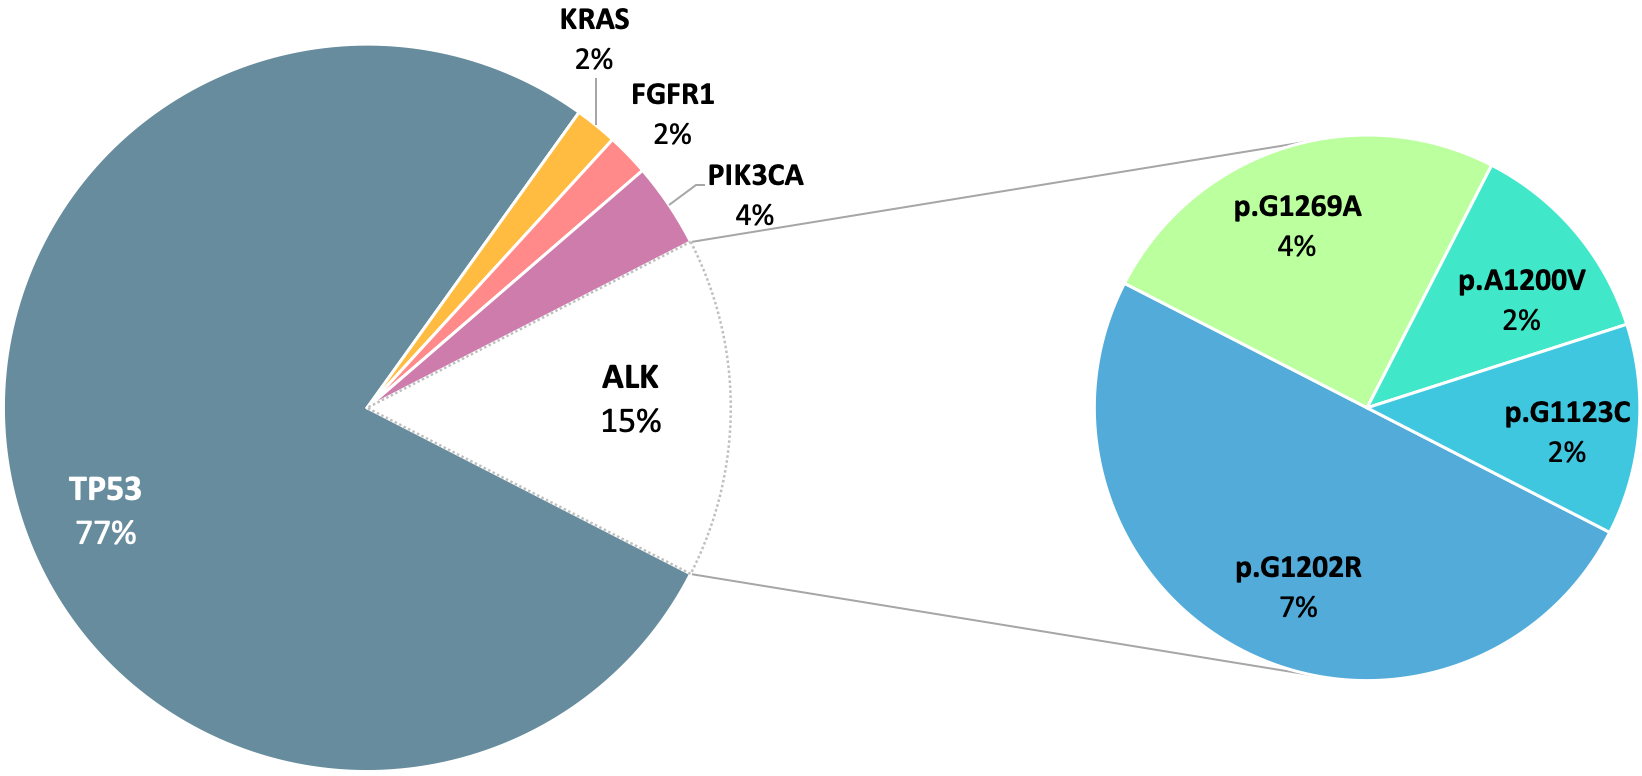
\includegraphics[width=0.9\textwidth]{Images/chapter_4/all_mutations.png}
    \caption{Frequency of the mutations identified in the study population, as well as the different types of ALK missense mutations.}
    \label{fig:All_mutations}
\end{figure}

In this context, 52 unique mutations were finally reported. As shown in \autoref{fig:All_mutations}, the most widely represented mutations occurred in the TP53 gene, with 40 cases. It was common to find multiple alterations of this type in the same sample and coexisting with ALK mutations, which are the target of this study. On the other hand, alterations were also detected in the PIK3CA, KRAS, and FGFR1 genes, appearing both individually and concurring with the rest of the detected variants. These mutations are found in more detail in \autoref{tab:TP53_Mutations}.

\begin{table}[t]
\centering
\resizebox{0.52\textwidth}{!}{
\renewcommand{\arraystretch}{1.3}
\begin{tabular}{cccc}
\rowcolor[HTML]{C0C0C0} 
\textbf{Gene}                                             & \textbf{\begin{tabular}[c]{@{}c@{}}Genomic\\ Alteration\end{tabular}} & \textbf{\begin{tabular}[c]{@{}c@{}}Nucleotide\\ Change\end{tabular}} & \textbf{\begin{tabular}[c]{@{}c@{}}Number of\\ Cases\end{tabular}} \\
\rowcolor[HTML]{FFFFFF} 
\cellcolor[HTML]{FFFFFF} & p.P92A & c.274C\textgreater{}G & 13 \\
\rowcolor[HTML]{EFEFEF} 
\cellcolor[HTML]{FFFFFF} & p.A88fs & c.261\_262insC & 4 \\
\rowcolor[HTML]{FFFFFF} 
\cellcolor[HTML]{FFFFFF} & p.R282W & c.844C\textgreater{}T & 3 \\
\rowcolor[HTML]{EFEFEF} 
\cellcolor[HTML]{FFFFFF} & p.V197fs & c.590delT & 1 \\
\rowcolor[HTML]{FFFFFF} 
\cellcolor[HTML]{FFFFFF} & p.M133T & c.398T\textgreater{}C & 1 \\
\rowcolor[HTML]{EFEFEF} 
\cellcolor[HTML]{FFFFFF} & p.H380fs & c.1140delT & 1 \\
\rowcolor[HTML]{FFFFFF} 
\cellcolor[HTML]{FFFFFF} & p.P359A & c.1075C\textgreater{}G & 1 \\
\rowcolor[HTML]{EFEFEF} 
\cellcolor[HTML]{FFFFFF} & p.R248Q & c.743G\textgreater{}A & 1 \\
\rowcolor[HTML]{FFFFFF} 
\cellcolor[HTML]{FFFFFF} & p.Y220C & c.659A\textgreater{}G & 1 \\
\rowcolor[HTML]{EFEFEF} 
\cellcolor[HTML]{FFFFFF} & p.S90fs & c.267\_268insC & 1 \\
\rowcolor[HTML]{FFFFFF} 
\cellcolor[HTML]{FFFFFF} & p.G105C & c.313G\textgreater{}T & 1 \\
\rowcolor[HTML]{EFEFEF} 
\cellcolor[HTML]{FFFFFF} & p.S15* & c.42\_43insT & 1 \\
\rowcolor[HTML]{FFFFFF} 
\cellcolor[HTML]{FFFFFF} & p.S149fs & c.445delT & 1 \\
\rowcolor[HTML]{EFEFEF} 
\cellcolor[HTML]{FFFFFF} & p.Q16fs & c.45delT & 1 \\
\rowcolor[HTML]{FFFFFF} 
\cellcolor[HTML]{FFFFFF} & p.V157F & c.469G\textgreater{}T & 1 \\
\rowcolor[HTML]{EFEFEF} 
\cellcolor[HTML]{FFFFFF} & p.R158C & c.472C\textgreater{}T & 1 \\
\rowcolor[HTML]{FFFFFF} 
\cellcolor[HTML]{FFFFFF} & p.M160I & c.480G\textgreater{}T & 1 \\
\rowcolor[HTML]{EFEFEF} 
\cellcolor[HTML]{FFFFFF} & p.C176Y & c.527G\textgreater{}A & 1 \\
\rowcolor[HTML]{FFFFFF} 
\cellcolor[HTML]{FFFFFF} & p.S241A & c.721T\textgreater{}G & 1 \\
\rowcolor[HTML]{EFEFEF} 
\cellcolor[HTML]{FFFFFF} & p.P250L & c.749C\textgreater{}T & 1 \\
\rowcolor[HTML]{FFFFFF} 
\cellcolor[HTML]{FFFFFF} & p.G262R & c.784insC & 1 \\
\rowcolor[HTML]{EFEFEF} 
\cellcolor[HTML]{FFFFFF} & p.R273Gly & c.817C\textgreater{}G & 1 \\
\rowcolor[HTML]{FFFFFF} 
\multirow{-23}{*}{\cellcolor[HTML]{FFFFFF}\textbf{TP53}}  & p.? & c.919+10C\textgreater{}T & 1 \\
\rowcolor[HTML]{EFEFEF} 
\cellcolor[HTML]{EFEFEF} & p.E545K & c.1633G\textgreater{}A & 1 \\
\rowcolor[HTML]{EFEFEF} 
\multirow{-2}{*}{\cellcolor[HTML]{EFEFEF}\textbf{PIK3CA}} & p.E545A & c.1634A\textgreater{}C & 1 \\
\rowcolor[HTML]{FFFFFF} 
\textbf{KRAS} & p.G12C & c.34G\textgreater{}T & 1 \\
\rowcolor[HTML]{EFEFEF}
\textbf{FGFR1} & p.T174fs & 520delA & 1
\end{tabular}}
\caption{TP53, PIK3CA, KRAS, and FGFR1 gene mutations identified in the study population and their prevalence.}
\label{tab:TP53_Mutations}
\end{table}

The average number of variants per patient was 1.7. However, 7 patients did not present any mutation and in 22 of them, no ALK alteration was found. Furthermore, there were no significant differences in the amount of cfDNA input between patients with and without an associated mutation. In this sense, only 1 subject had a single ALK mutation, while the remaining 7 patients had it coexisting with alterations in the TP53 gene.

The ALK variants confirmed by dPCR are represented in \autoref{tab:ALK_dPCR}. As can also be seen in \autoref{fig:All_mutations}, the most prevalent mutation was G1202R, identified in 4 different patients who had progressed on alectinib (N$=$3) and ceritinib (N$=$1). The G1123C mutation (N$=$1) also arose as a result of the failure of a second-generation inhibitor. The remaining G1269A (N$=$2) and A1200V (N$=$1) alterations were detected upon progression to crizotinib. Furthermore, these mutations were detected at a median MAF of 0.4\%.

\begin{table}[ht]
\centering
\resizebox{0.7\textwidth}{!}{
\renewcommand{\arraystretch}{1.3}
\begin{tabular}{ccccc}
\rowcolor[HTML]{C0C0C0} 
\textbf{\begin{tabular}[c]{@{}c@{}}Patient\\ ID\end{tabular}} & \textbf{\begin{tabular}[c]{@{}c@{}}Nucleotide\\ Change\end{tabular}} & \textbf{\begin{tabular}[c]{@{}c@{}}Amino Acid\\ Change\end{tabular}} & \textbf{\begin{tabular}[c]{@{}c@{}}Progression\\ to\end{tabular}} & \textbf{\begin{tabular}[c]{@{}c@{}}MAF\\ (dPCR)\end{tabular}} \\
\rowcolor[HTML]{FFFFFF} 
ARS\_1 & p.G1269A & c.3806G\textgreater{}C & Crizotinib & 0.42\% \\
\rowcolor[HTML]{EFEFEF} 
ARS\_2 & p.G1202R & c.3604G\textgreater{}A & Ceritinib & 2.12\% \\
\rowcolor[HTML]{FFFFFF}
AHT & p.A1200V & c.3599C\textgreater{}T & Crizotinib & - \\
\rowcolor[HTML]{EFEFEF}
AMLO & p.G1269A & c.3806G\textgreater{}C & Crizotinib & 2.80\% \\
\rowcolor[HTML]{FFFFFF} 
GCP & p.G1123C & c.3367G\textgreater{}T & Alectinib & - \\
\rowcolor[HTML]{EFEFEF} 
MCPA & p.G1202R & c.3604G\textgreater{}A & Alectinib & 0.40\% \\
\rowcolor[HTML]{FFFFFF} 
MESR & p.G1202R & c.3604G\textgreater{}A & Alectinib & 0.30\% \\
\rowcolor[HTML]{EFEFEF} 
MSCS & p.G1202R & c.3604G\textgreater{}A & Alectinib & 0.01\% 
\end{tabular}}
\caption{Characteristics of the ALK mutations identified in this study.}
\label{tab:ALK_dPCR}
\end{table}

On the other hand, in 12 patients only TP53 mutations could be confirmed, in 1 individual concurrence of alterations in PIK3CA and TP53 was found, in another only 1 variant of PIK3CA was detected, and the last patient had mutations in the FGFR1, KRAS, and TP53 genes.

Regarding the different types of the verified variants, they are summarized at a cohort level in \autoref{fig:Waterfall} along with the main clinical characteristics of the patients. In this context, 14 subjects (46.7\%) were identified with multiple alterations. The most frequent mutation type was missense SNPs, detected in 40 different cases (29 in TP35, 8 in ALK, 2 in PIK3CA, and 1 in KRAS). Additionally, 12 InDels were also identified (11 in TP35 and 1 in FGFR1).

\begin{figure}[ht]
    \centering
    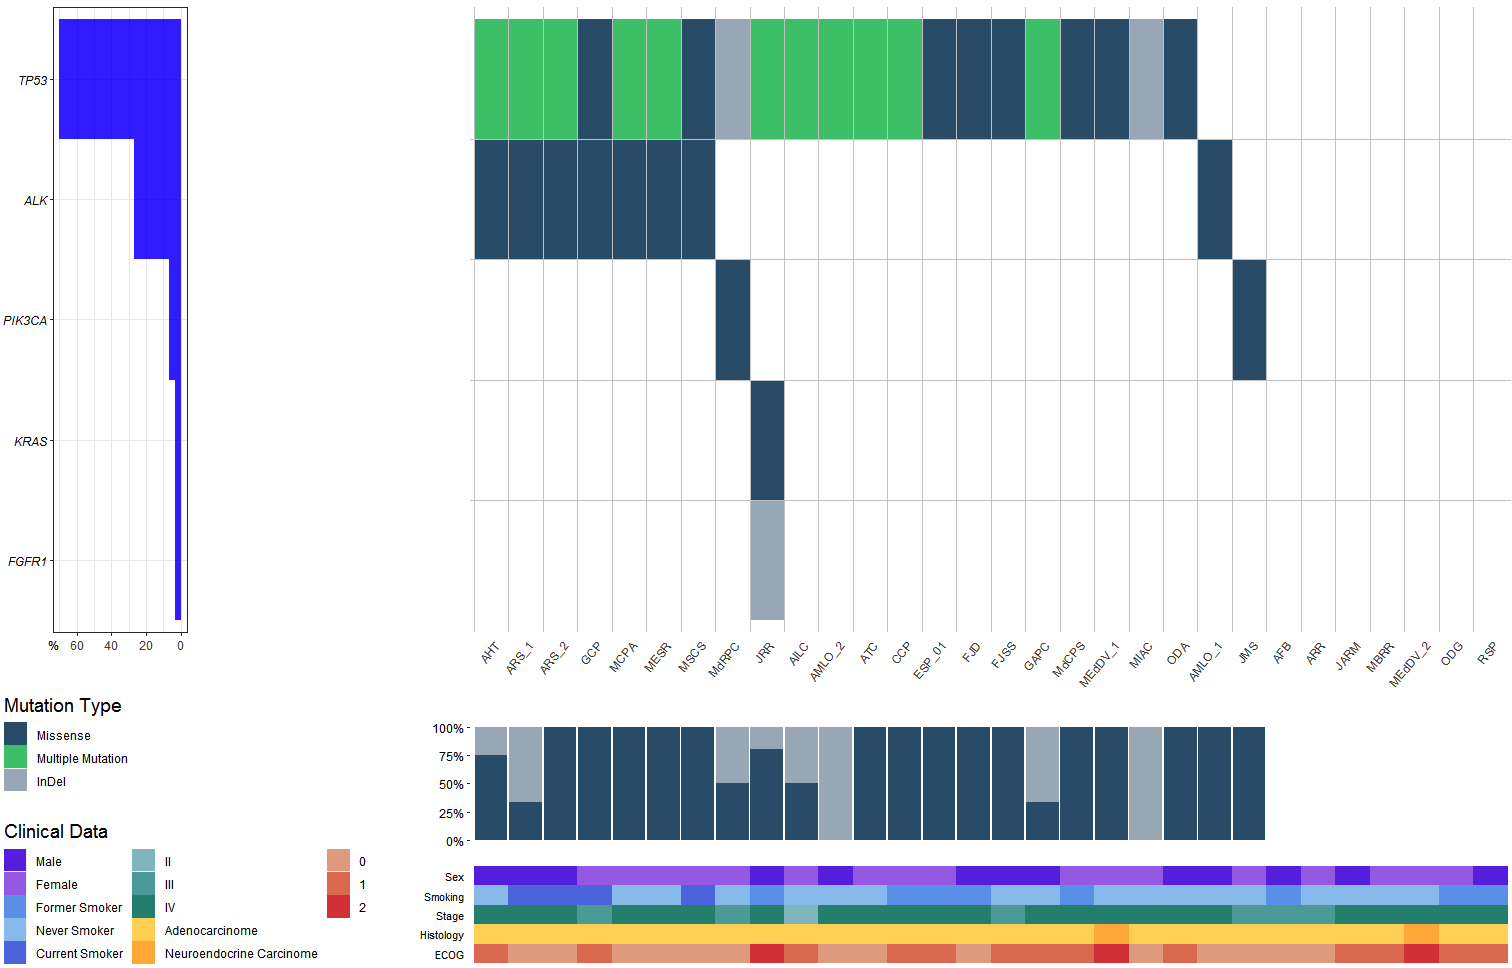
\includegraphics[width=\textwidth]{Images/chapter_4/waterfall.png}
    \caption{Co-mutation plot of the subjects of this study and their corresponding somatic mutations. The clinical features of each of the patients (gender, smoking status, diagnostic stage, histology, and ECOG performance status) and the characteristics of their mutations (type, prevalence, and associated gene) are shown. The multiple alterations class appear broken down into the subtypes that compose it.}
    \label{fig:Waterfall}
\end{figure}

Finally, all these results, and especially the confirmed positive (N$=$8) and negative (N$=$19) variants associated with the ALK mutations, were used to adjust the different parameters of the implemented algorithm.

\section{Implemented Pipeline}

The development of the bioinformatic pipeline was divided into two steps: the implementation of the filtering algorithm itself; and that of a graphical interface to simplify the process of selecting parameters and saving the output variants along with their properties in a \textit{.csv} file.

\subsection{Algorithm Characterization}

In order to detect all variants at the ALK gene locus, specific conditions for each of them were established from a set of previously validated samples. The flowchart in \autoref{fig:Algorithm} shows the basic structure of the developed pipeline and the selection criteria based on certain variables as presented in the \textit{non-filtered-oncomine.tsv} file.

\begin{figure}[ht]
    \centering
    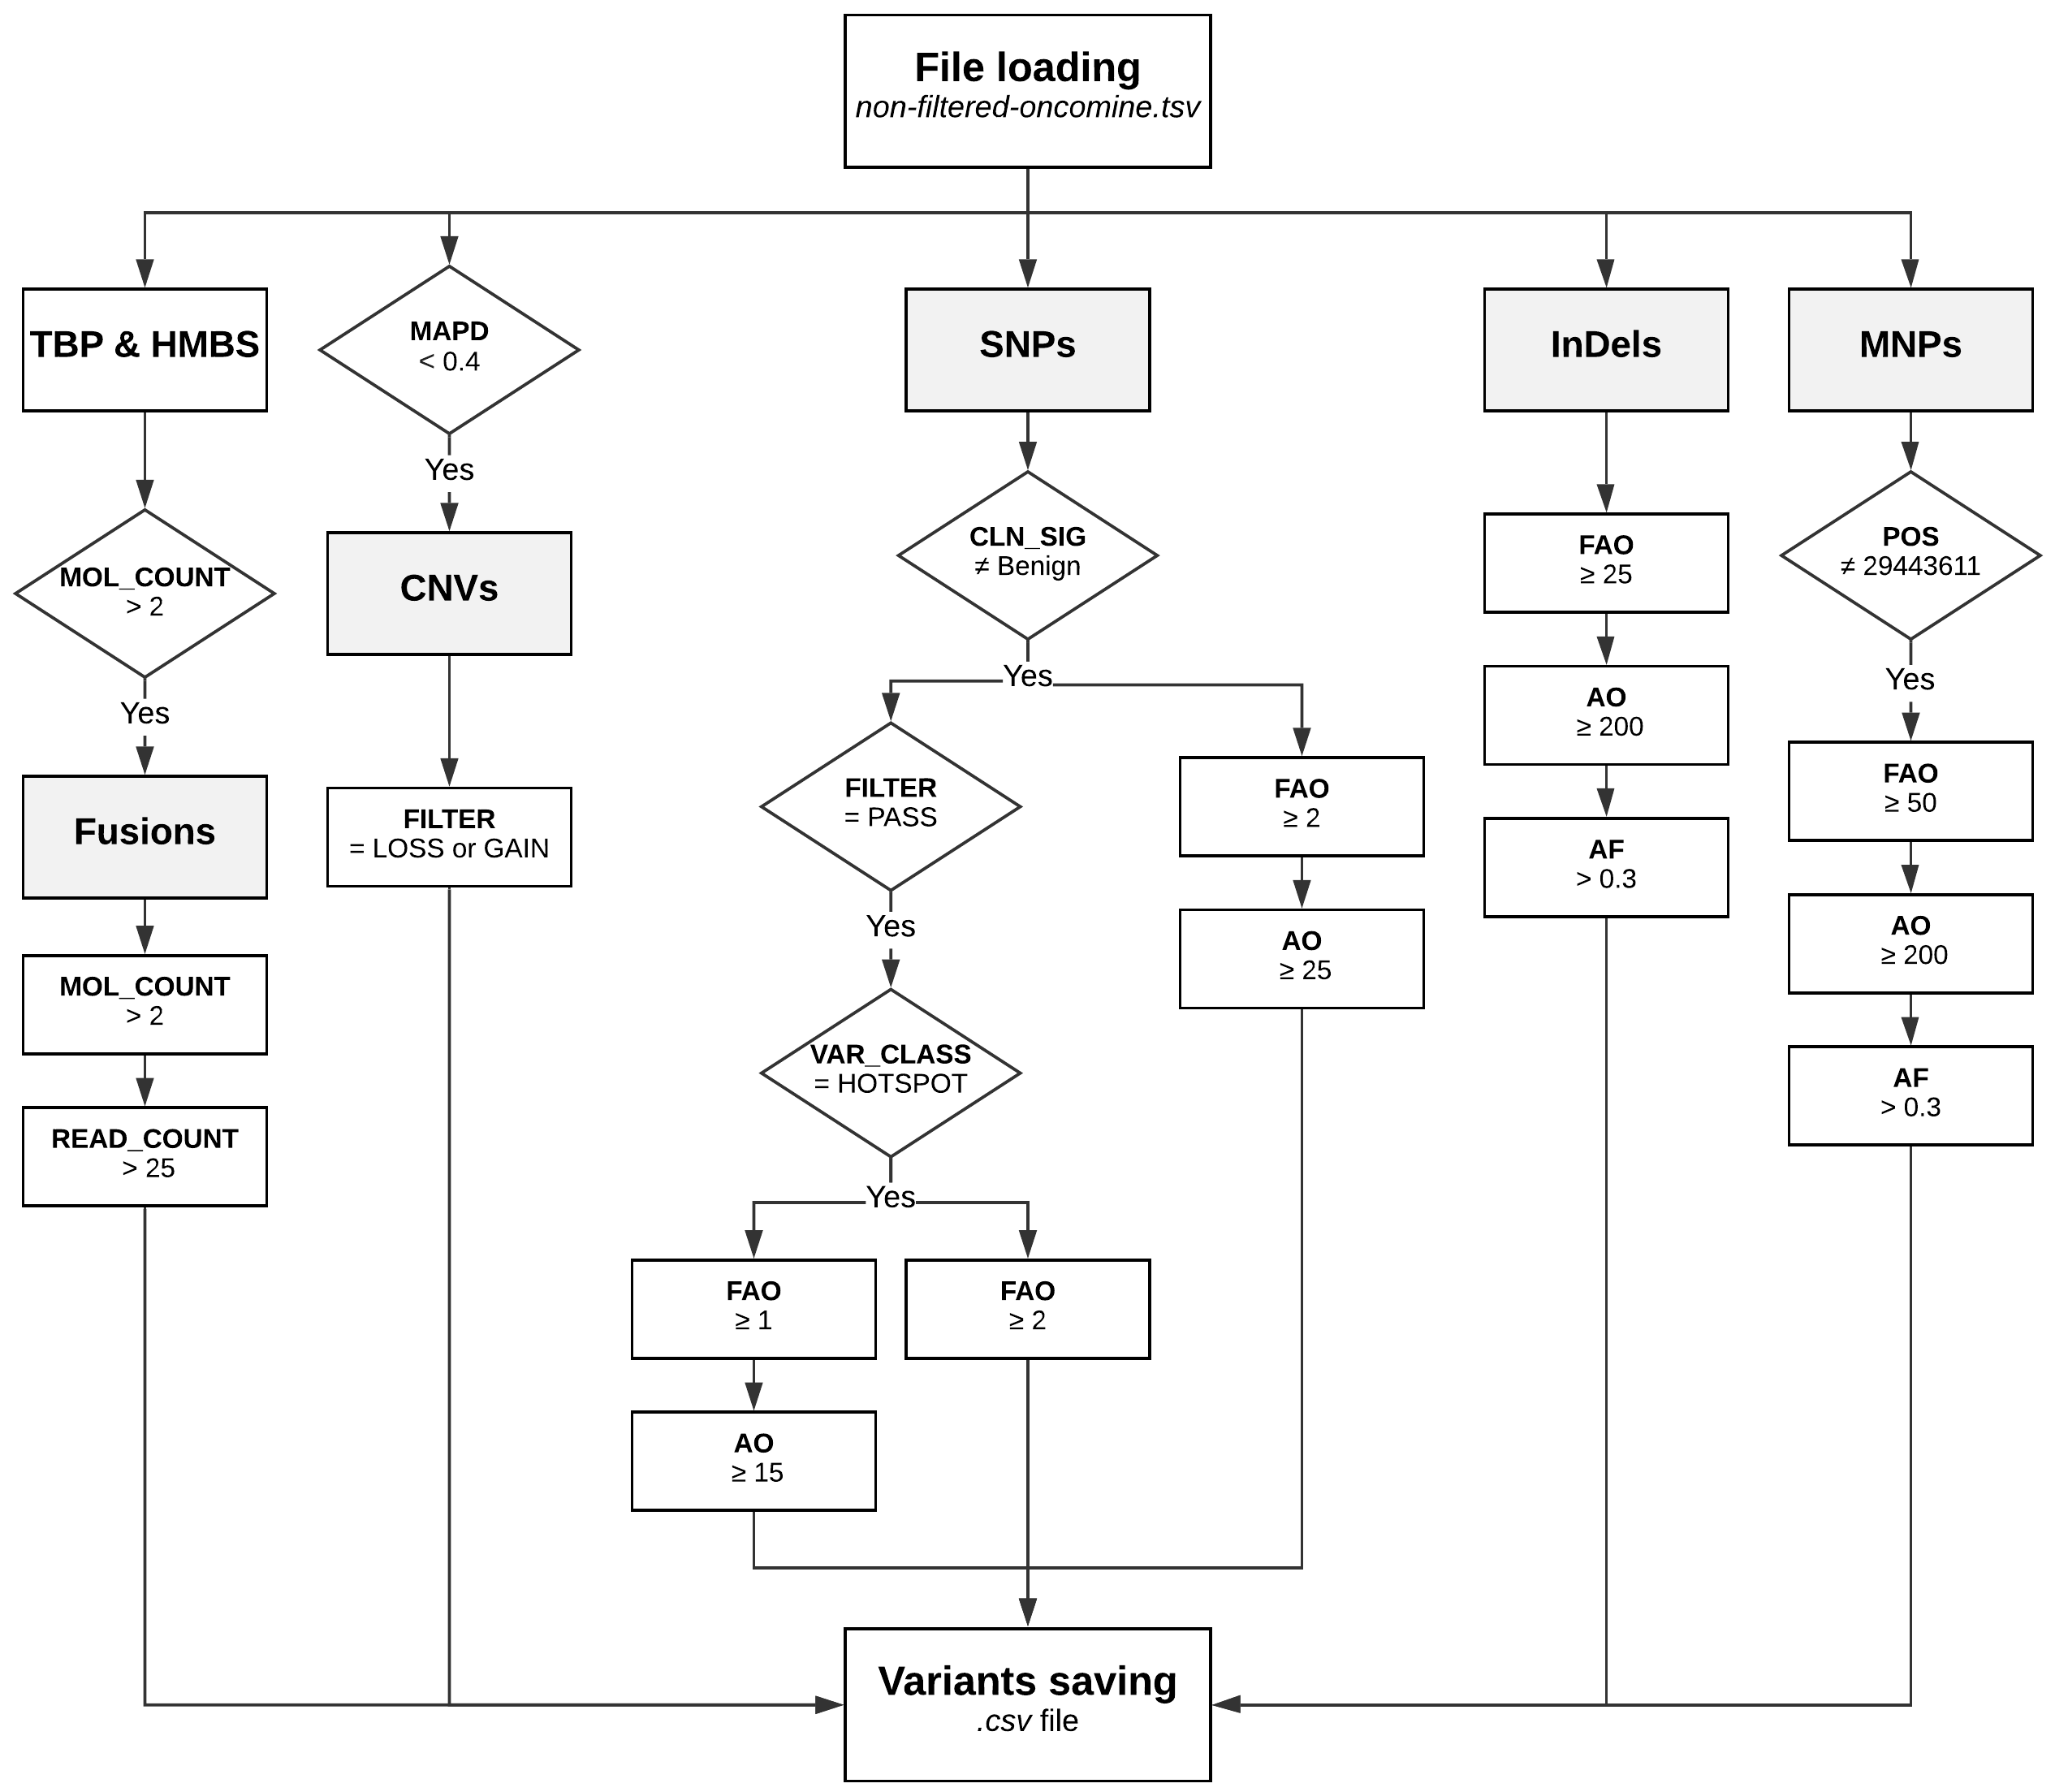
\includegraphics[width=\textwidth]{Images/chapter_4/mut_filtering.png}
    \caption{Flowchart of the bioinformatic pipeline optimized for the processing and assessment of variants at the ALK gene locus. MOL\_COUNT, molecular coverage; READ\_COUNT, read coverage; MAPD, median of the absolute values of all pairwise differences; FILTER: Ion Reporter\texttrademark{} internal filter (Oncomine\texttrademark{} Variants v5.12); CLN\_SIG, clinical significance; VAR\_CLASS: Oncomine\texttrademark{} Variant Class; POS: variant position; AF, allele frequency.}
    \label{fig:Algorithm}
\end{figure}

\subsubsection{Fusions Filtering}

The fusions filter selects translocations at the ALK locus with molecular coverage $> 2$, and fusion reads $> 25$. These thresholds were established according to the clinical study data and the Oncomine\texttrademark{} Pan‐Cancer Cell‐Free Assay recommendations.

Additionally, two control genes were included in each sequencing process to measure the transcript abundance, TATA-binding protein (TBP) and hydroxymethylbilane synthase (HMBS). Both must have molecular coverage $> 2$ to validate the filtered fusion variants by ensuring their correct amplification.

\subsubsection{Copy-Number Variations Filtering}

Following the Ion Reporter\texttrademark{} recommendations, to make a CNV call the median of the absolute values of all pairwise differences (MAPD) must be $< 0.4$. MAPD measures the absolute difference between the $log_2$ copy-number ratios of adjacent amplicons and then calculates the median across all wells (\autoref{eq:MAPD}).
\begin{align} \label{eq:MAPD}
    MAPD &= median(\mid x_{i+1}-x_i \mid) \\
    \text{where}~
    x_i &\equiv \text{$log_2$ ratio for marker i} \notag
\end{align}

Larger MAPD values indicate lower coverage uniformity and greater noise, resulting in a higher probability of erroneous CNV calls. Therefore, only samples showing an MAPD $< 0.4$ were considered in further analysis, which consisted of selecting ALK gene copy-number gains or losses.

\subsubsection{Single-Nucleotide Polymorphisms Filtering}

Taking into account that false positives of this type of variants are not common, the proposed algorithm makes a call as long as any of the following conditions is met, discarding variants with a benign or likely benign clinical significance:
\begin{itemize}
    \item SNPs in hotspot regions that have passed the Oncomine\texttrademark{} Variants v5.12 filter and that have been detected in at least 1 molecular count with $\ge 15$ reads.
    \item SNPs in hotspot regions that have passed the Oncomine\texttrademark{} Variants v5.12 filter and that have been detected in at least 2 molecular counts.
    \item SNPs that have been detected in at least 2 molecular counts with $\ge 25$ reads.
\end{itemize}

\subsubsection{Insertions and Deletions Filtering}

The sequencing results usually present doubtful data regarding InDels. Therefore, the restrictions are more severe for this filter, which selects only variants that have been detected in at least 25 molecular counts with $\ge 200$ reads and an allele frequency (AF) $\ge 0.03$.

\subsubsection{Multiple-Nucleotide Polymorphisms Filtering}

Based on data from confirmed ALK-positive samples, false positives are highly likely in MNPs. In this context, only variants that have been detected in at least 50 molecular counts with $\ge 200$ reads and an AF $\ge 0.03$ were considered for confirmation by dPCR. 

On the other hand, abnormal Ion GeneStudio\texttrademark{} S5 Sequencer behavior at position chr2:29443611 of the ALK locus and involving the reading of 6 consecutive guanines (G) was observed. Thus, variants at that location were excluded from further analysis.

\subsection{Graphical User Interface (GUI)}

The implemented user interface were developed to facilitate data input and interpretation of results. The different layouts are shown in \autoref{fig:GUI}.

\begin{figure}[ht]
    \centering
    \begin{subfigure}{\textwidth}
        \centering
        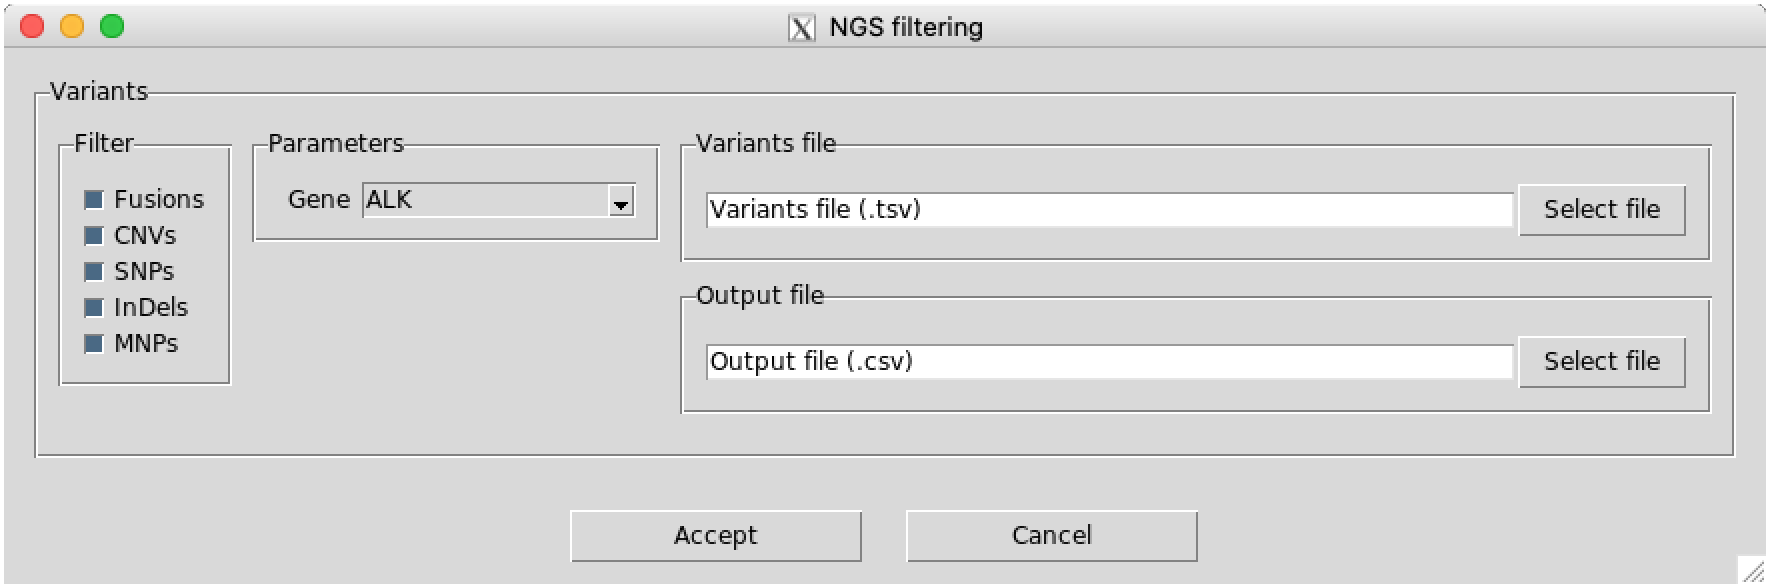
\includegraphics[width=\textwidth]{Images/chapter_4/GUI_1.png}
        \caption{Start screen. It allows selecting the type of variant\slash s to filter, the gene involved (ALK currently), as well as the source and output files. \\}
        \label{fig:GUI_1}
    \end{subfigure}
    \hfill
    \begin{subfigure}{0.47\textwidth}
        \centering
        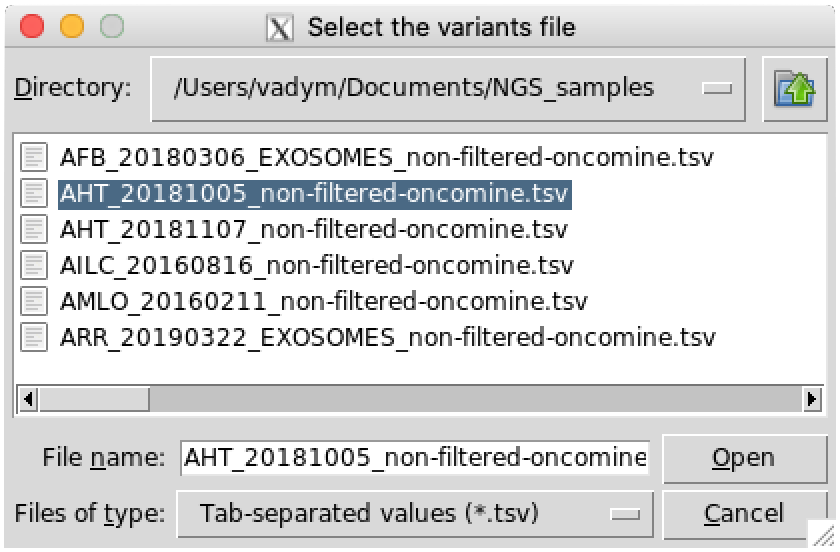
\includegraphics[width=\textwidth]{Images/chapter_4/GUI_2.png}
        \caption{Pop-up window for selecting the \textit{.tsv} source file containing raw variants.}
        \label{fig:GUI_2}
    \end{subfigure}
    \hfill
    \hfill
    \begin{subfigure}{0.52\textwidth}
        \centering
        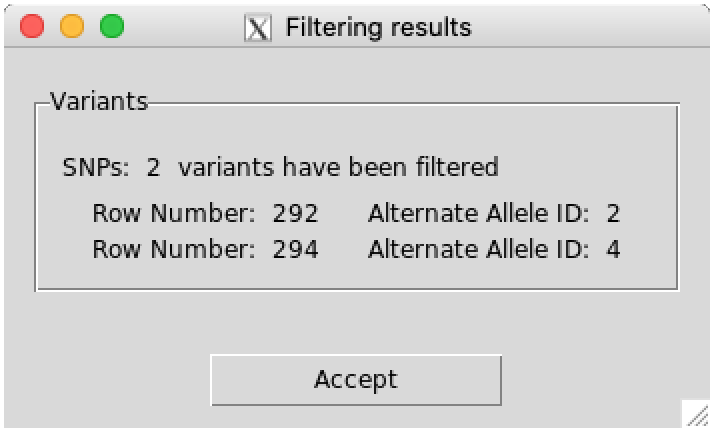
\includegraphics[width=\textwidth]{Images/chapter_4/GUI_3.png}
        \caption{Results screen showing 2 filtered SNPs and their $.tsv$ row number and alternate allele ID.}
        \label{fig:GUI_3}
    \end{subfigure}
    \hfill
    \caption{Implemented GUI showing the different display areas that appear throughout the filtering process.}
    \label{fig:GUI}
\end{figure}

The start screen (\autoref{fig:GUI_1}) has several options that allow some variability when proceeding with the filtering process. On the one hand, it is possible to select the filter\slash s to apply to the \textit{non-filtered-oncomine.tsv} file, as well as the gene to study. Currently, and as previously described, only the ALK gene has been addressed. On the other hand, the user can select both the source and output files through a pop-up screen, which is shown in \autoref{fig:GUI_2}. In case the output file does not exist, the program creates it automatically.

Finally, to fully characterize the variants that have passed a particular filter, the results are displayed specifying the mutation type, the row number of the variants in the \textit{non-filtered-oncomine.tsv} file, and the identifier of the alternate allele (\autoref{fig:GUI_3}). Simultaneously, each of the identified variants is appended to the $.csv$ output file along with its main characteristics.

It should also be noted that several additional screens have been implemented to offer the end-user information on the progress of the filtering process, on any errors that may have occurred during it, and on the non-identification of any variant of interest by the algorithm.

\section{Performance of the Implemented Algorithm}

The 39 initial sequenced samples were used to study the performance of the developed algorithm regarding the ALK mutations confirmed by dPCR, which was considered the gold standard. To asses this, sensitivity, specificity, and positive and negative predictive values, shown in \autoref{tab:ALG_performance}, were calculated based on the 30 patients in this study. Furthermore, a prevalence of ALK mutations of 20\% was assumed for these calculations since approximately 20–50\% of patients treated with an ALK inhibitor end up developing some type of resistance \cite{TKI_resistance, ALK_resistance}. 

\begin{table}[ht]
\centering
\resizebox{0.75\textwidth}{!}{
\renewcommand{\arraystretch}{1.3}
\begin{tabular}{lcc}
\rowcolor[HTML]{C0C0C0} 
\multicolumn{1}{c}{\cellcolor[HTML]{C0C0C0}\textbf{Statistic}} & \textbf{Value} & \textbf{95\% CI}   \\
\rowcolor[HTML]{FFFFFF} 
Sensitivity & 87.50\% & 47.35\% to 99.68\% \\
\rowcolor[HTML]{EFEFEF} 
Specificity & 81.82\% & 59.72\% to 94.81\% \\
\rowcolor[HTML]{FFFFFF} 
Disease prevalence & 20.00\% & - \\
\rowcolor[HTML]{EFEFEF} 
Positive Predictive Value & 54.61\% & 32.31\% to 75.20\% \\
\rowcolor[HTML]{FFFFFF} 
Negative Predictive Value & 96.32\% & 80.55\% to 99.40\% \\
\rowcolor[HTML]{EFEFEF} 
Accuracy & 82.95\% & 64.83\% to 94.13\%
\end{tabular}}
\caption{Performance of the algorithm developed to filter the ALK mutations obtained from NGS. The results obtained by dPCR were taken as the gold standard.}
\label{tab:ALG_performance}
\end{table}

In this context, the algorithm managed to successfully identify 7 of the 8 mutations confirmed by dPCR, reaching a specificity of 87.50\%. Specifically, the $AHT$ patient sample was discarded by the algorithm (\autoref{tab:ALK_dPCR}). On the other hand, 4 patients were incorrectly classified as carriers of ALK mutations, thus a specificity of 81.82\% was obtained. Finally, the algorithm reported an accuracy of 82.95\%, with a remarkable performance in terms of discarding samples without any mutation since a negative predictive value of 96.32\% was achieved.

Noteworthy, the Oncomine\texttrademark{} Variants v5.12 filter only detected ALK mutations in 3 patients.








%%%%%%%%%%%%%%%%%%%%%%%%%%%%%%%%%%%%%%%%%%%%%%%%%%%%%%%%%%%%%%%%%%%%%%%%
% ALK white type 22

% 7 pacientes no presentaban ninguna mutación
% 1 paciente solo con ALK
% 7 pacientes con ALK + TP53
% 12 pacientes solo con TP53
% 1 paciente con PIK3CA + TP53
% 1 paciente PIK3CA
% 1 paciente con FGFR1 + KRAS + TP53

%%%%%%%%%%%%%%%%%%%%%%%%%%%%%%%%%%%%%%%%%%%%%%%%%%%%%%%%%%   TOTAL = 30

% MUTACIONES/SAMPLEs %%%%%%%%%%%%%%%%%%%%%%%%%%%%%%%%%%%%%%%%%%%%%%%%%%%%

    % 11 patients with multiple TP53 mutations
    % 3 patients with InDels
        % 1 FGFR1
        % 2 TP53
    % 8 patients with ALK SNPs
    % 8 patients with TP53 SNPs
    % 1 patients with KRAS SNPs
    % 2 patients with PIK3CA SNPs

%%%%%%%%%%%%%%%%%%%%%%%%%%%%%%%%%%%%%%%%%%%%%%%%%%%%
% 40 missenses
% 12 indles

% ALK: 8 + 1 missenses
% FGFR1: 1 indel
% KRAS: 1 messense
% PIK3CA: 2 missenses
% TP53: 
%     2 indels
%     8 missenses
%     *11* multiple mutations
%           21+1 missenses
%           9 indels
%%%%%%%%%%%%%%%%%%%%%%%%%%%%%%%%%%%%%%%%%%%%%%%%%%%%%%%%%%  TOTAL = 52+2


% MUTACIONES/SAMPLEs %%%%%%%%%%%%%%%%%%%%%%%%%%%%%%%%%%%%%%%%%%%%%%%%%%%%%%
% POR IGV %%%%%%%%%%%%%%%%%%%%%%%%%%%%%%%%%%%%%%%%%%%%%%%%%%%% 40
    % 1 FGFR1
    % 19 + 1 (misma mutación) + 19 (naranja) TP53 %%%%  39
% POR DPCR %%%%%%%%%%%%%%%%%%%%%%%%%%%%%%%%%%%%%%%%%%%%%%%%%%%% 14
    % 8 + 1 (hay una misma mutación),  ALK (LA ROSA NO SE CUENTA)
    % 0 (en la azul no queda material) + 2 TP53
    % 2 PIK3CA
    % 1 KRAS
%%%%%%%%%%%%%%%%%%%%%%%%%%%%%%%%%%%%%%%%%%%%%%%%%%%%%%%%%%   TOTAL = 54